\documentclass[a4paper, 12pt]{article}

\usepackage{graphicx}
\usepackage{xcolor}
\usepackage{mdframed}
\usepackage { amsmath , amssymb , amsthm }
\usepackage[T2A]{fontenc}
\usepackage[utf8]{inputenc}
\usepackage[english,russian]{babel}

\graphicspath{{img/}}
\DeclareGraphicsExtensions{.pdf,.png,.jpg}


\title{Инженерная графика}
\author{Щербинин В.В}
\date{\today}

\begin{document}
\sffamily
\maketitle

\section*{Введение}

ЕСКД -- единая система конструкторской документации (устанавливает взаимосвязь правил по оформлению, конструированию, обращинию конструкторской документации)\\
"+":\\
1. Возможность взаимообмена конструкторской документации между предприятиями.\\
2. Стабилизация комплектности, исключающая дубрированость документов.\\
3. Возможность обеспечивать унификации при конструировании, разработке, проэктированиии комерческих изделий\\
4. Упращенная форма конструкторской документации.\\
5. Механизм и автоматизм обработки технической документации.\\
\newpage
\section{Методы проекции}

\subsection{Центральная проекция}
Для получения центральных проекций необходимо задаться плоскостью проекций H и центром проекций S.\\
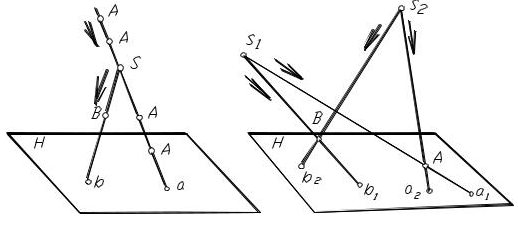
\includegraphics{eng1}\\
Центр проекций действует как точечный источник света, испуская проецирующие лучи. Точки пересечения проецирующих лучей с плоскостью проекций H называются проекциями. Проекций не получается, когда центр проецирования лежит в данной плоскости или проецирующие лучи параллельны плоскости проекций.\\

Свойства центрального проецирования:\\
1.Каждая точка пространства проецируется на данную плоскость проекций в единственную проекцию.\\
2.В то же время каждая точка на плоскости проекций может быть проекцией множества точек, если они находятся на одном проецирующем луче\\
3.Прямая, не проходящая через центр проецирования, проецируется прямой (проецирующая прямая – точкой).\\
4.Плоская (двумерная) фигура, не принадлежащая проецирующей плоскости, проецируется двумерной фигурой (фигуры, принадлежащие проецирующей плоскости, проецируются вместе с ней в виде прямой).\\
5.Трехмерная фигура отображается двумерной.\\
Глаз, фотоаппарат являются примерами этой системы изображения. Одна центральная проекция точки не дает возможность судить о положении самой Точки в пространстве, и поэтому в техническом черчении это проецированиепочти не применяется. Для определения положения точки при данном способе необходимо иметь две ее центральные проекции, полученные из двух различных центров. Центральные проекции применяют для изображения предметов в перспективе. Изображения в центральных проекциях наглядны, но для технического черчения неудобны.

\subsection{Параллельная проекция и их свойства}
Параллельное проецирование – частный случай центрального проецирования, когда центр проецирования перемещен в несобственную точку, т.е. в бесконечность. При таком положении центра проекций все проецирующие прямые будут параллельны между собой. В связи с параллельностью проецирующих прямых рассматриваемый способ называется параллельным, а полученные с его помощью проекции – параллельными проекциями. Аппарат параллельного проецирования полностью определяется положением плоскости проецирования (H) и направлением проецирования.\\

Свойства параллельного проецирования:\\
1.При параллельном проецировании сохраняются все свойства центрального проецирования, а также возникают новые:\\
2.Для определения положения точки в пространстве необходимо иметь две ее параллельные проекции, полученные при двух различных направлениях проецирования.\\
3.Параллельные проекции взаимно параллельных прямых параллельны, а отношение длин отрезков таких прямых равно отношению длин их проекций.\\
4.Если длина отрезка прямой делится точкой в каком-либо отношении, то и длина проекции отрезка делится проекцией этой точки в том же отношении .\\
5.Плоская фигура, параллельная плоскости проекций , проецируется при параллельном проецировании на эту плоскость в такую же фигуру.\\

Параллельное проецирование, как и центральное, при одном центре проецирования, также не обеспечивает обратимости чертежа.\\
Применяя приемы параллельного проецирования точки и линии, можно строить параллельные проекции поверхности и тела.\\

\subsection{Прямоугольное (ортогональное)проецирование}

\textbf{Прямоугольное проецирование} -- это частный случай параллельного проец при котором проецирующие прямые перпендикулярны плоскости проекции и параллельны друг-другу.
\\
Ортогональные проекции двух взаимно перпендикулярных прямых, одна из которых параллельны плоскоти проекций а другая не перпендикулярна ей взаимно перпендикулярны.\\
Преймущества:\\
1. простота\\
2. при ортогональном проецировании, при ряди условий удается сохранить форму и размеры фигуры.\\

\subsection{Проецирование на две взаимно перпендикулярные плоскости проекции}
Обратимость чертежа может быть обеспечена проецированием на две плоскости проекции.\\

Состоит из фронтальной и горезонтальной плоскастей проекций, а линия пересечения называется осью проекции и называбт x или v/h.\\
%вставить рисунок взаимно перпендикулярных плоскостей

В некоторых случаях удобней использовать\\
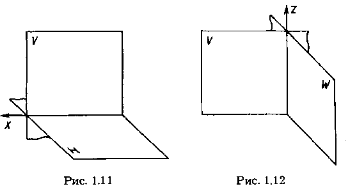
\includegraphics{143}\\
состоит из фронтальной и профильной плоскотей проекций, ось пересечения называется v/w.\\

Горизонтальные проекции точки называют прямоугольную проекцию точки на горизонтальную плоскость проекции.\\
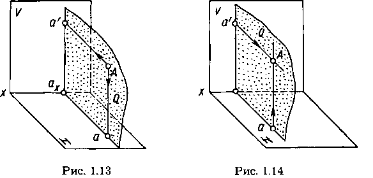
\includegraphics{eng141}\\
%вставить рисунок проецирования v/h
обозначения: $ a $ на h , $ a' $ на v для точки $ A $\\
плоскость Q перпендикулярна плоскостям проекции и пересекает ось проекции x\\
Для того чтобы востановить положение A необходимо востановить перпендикуляры к плоскостям проекций в $a \quad a'$, на пересечении перпендикуляров находится точка A\\
Две параллельные проекции точки на различные плоскости проекции вполне определяют ее положение в пространстве, а значит проецирование на две ортогональных плоскости проекции обеспечивает обратимость чертежа для точки.\\

Эпюры Моджа:\\
%рисунок
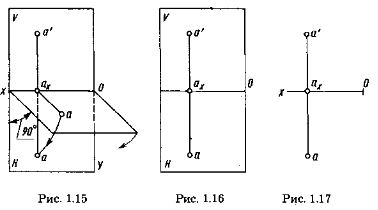
\includegraphics{142}\\
Отрезок a'a называетс линией связи\\

\subsection{Проецирование на три взаимно перпендикулярные плоскости проекции}

%рисунок трех плоскостей проекции
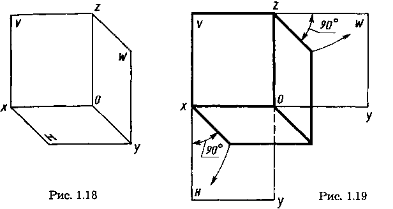
\includegraphics{151}
называется V,H,W. Точка O - пересечение трех проекций.\\

Принято разрезать ось y\\

!!!Помнить про чертову прямую -45 градусов\\
При параллельных прямых все их проекции параллельны!!!\\

\section{Глава. Проецирование отрезка прямой линии}
\subsection{Проецирование отрезка прямой линии и деление его в заданном отношении}

Отрезки $a_p \quad b_p$ ледат в некоторой плоскости Q, эта плоскость перпендикулярна плоскости P, прямая, по которой плоскость Q пересекает плоскость P содержит точки AB\\
\begin{center}
	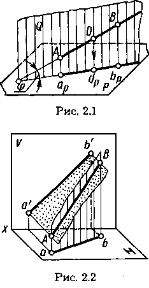
\includegraphics{img/211.png}
\end{center}


если точка принадлежит никакому отношению то ее проекции принадлежат одноименным проекциям отрезка и делят их в одном и томже отношении.
\\

\subsection{Положение прямой линии относительно плоскостей проекции. Особые случаи положения прямой}
1. прямая не параллельна ни одной из плоскостей проекции(прямая общего положения)\\
2. прямая параллельны одной из плоскостей проекции или ей принадлежит(прямая частного положения)\\
3. параллельна двум плоскостям проекции и перпендикулярна третей(прямая частного положения)\\
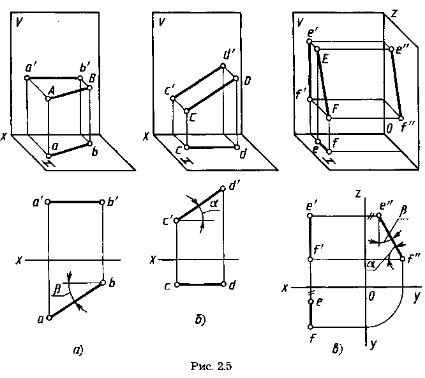
\includegraphics{img/221.png}\\
Соответственно называется фронтальной или профильной прямой(в зависимости какой параллельна плоскости).\\
Если прямая перпендикулярна одной из плоскостей проекции то она называется проецирующей для этой плоскости(горизонтально,фронтально,профильно проецирующией)\\
Проецирующая прямая проецируется на соответствующиую плоскость проекции в точку.\\

\subsection{Определение натуральной велечины прямой, общего положения и углов его наклона к плоскостям проекции}
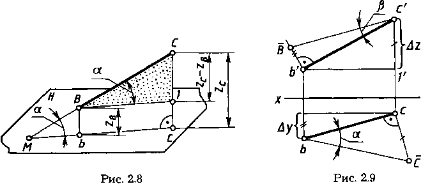
\includegraphics{img/231.png}\\
Итак, натуральную величину отрезка определяют как гипотенузу прямоугольного треугольника, одним из катетов которого является горизонтальная (фронтальная) проекция отрезка, другим — разность координат концов отрезка до горизонтальной (фронтальной) плоскости проекций. Этот метод иногда называют способом прямоугольного треугольника.\\
Угол между прямой и плоскостью проекций определяется как угол между прямой и ее проекцией на эту плоскость
\subsection{Взаимное положение прямой}
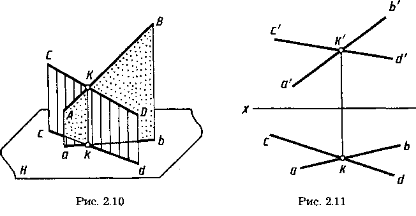
\includegraphics{img/241.png}\\
Пересекающиеся прямые -- если прямые пересекаются то их одноименные проекции персекаются между собой а проекции точек пересечения лежат на одной линии связи. В системе VH справедливо для всях прямых кроме профильных и обратное утверждение, если точки пересечения одноименных проекций прямых лежат на одной линии связи то прямые пересекаются.\\
\[
	\frac{b' m'}{a' m'} = \frac{b m}{a m}	
\]
\[
	\frac{c' m'}{a' m'} = \frac{cm}{am}	
\]
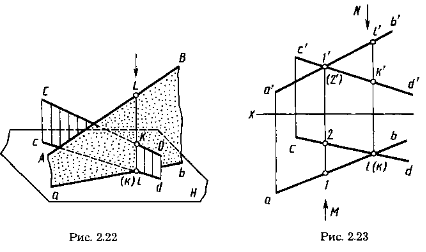
\includegraphics{img/242.png}\\
Параллельные прямые -- если прямые параллельны то их одноименные проекции параллельны между собой. Для прямых общего положения справедливо и обратное, если проекции прямых общего положения в системе двух плоскостей проекции параллельны то сами прямые также параллельны. Если одноименные проекции прямых параллельны одной из осей проекции то прямые параллельны при условии параллельности одноименных проекций на той плоскости проекций которой параллельны прямые.\\
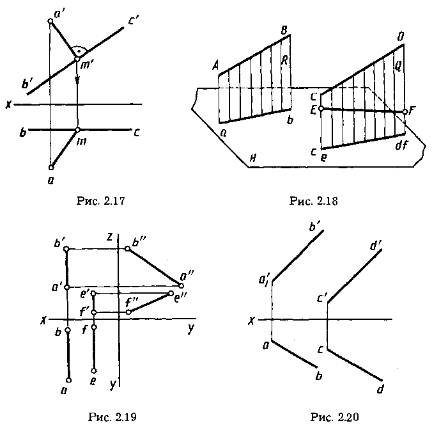
\includegraphics{img/243.png}\\
Скрещивающиеся прямые не имеют общих точек. Проекции скрещивающихся прямых пересекаются но точки пересечения проекций не лежат на одной линии связи.\\

\section{Глава. Плоскость}
\subsection{Положение плоскости относительно плоскостей проекции}

Плоскость можно задать разными способами:\\
-3мя точками, нележащими на одной прямой\\
-прямой и точкой, взятой вне этой прямой\\
-двумя пересекающимися прямыми\\
-двумя параллельными прямымы\\
-какая-либо плоская фигура\\

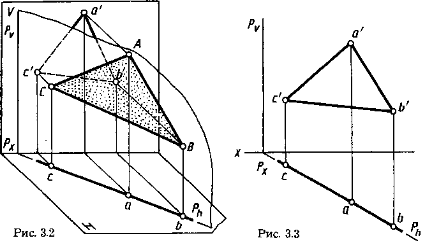
\includegraphics{img/311.png}\\
Положение плоскости по отношению к плоскотям проекции:\\
1)Плоскость не перпендикулярны плоскостям проекций(плоскость общего положения)\\
2)плоскость может быть перпендикулярна одной плоскости проекции(плоскости часного положения, проецирующие плоскости)\\
3)плоскость может быть перпендикулярна двум плоскостям проекции(плоскости часного положения, проецирующие плоскости)\\

След плоскости -- это линия пересечения плоскости с плоскостью проекции.\\

Для плоскости перпендикулярной плоскости H горизонтальный след PH распологается под углом к оси проекции X соответсвующе углу наклона этой плоскости к фронтальной плоскости проекции, а фронтальный след перпендикулярно оси X. Для плоскости перпендикулярной плоскости V фронтальный след распологается под углом к оси x соотвествующим углу наклона этой плоскости к плоскости H а горизонтальный след перпендикулярен оси X. На чертежах след перпендикулярный оси проекции не изображают.\\

Любая геометрическая фигура, лежащая в проецирующей плоскости, проецируется на соотвествующую плоскость проекции в прямую линию.\\
Плоскость перпендикулярна двум плоскостям проекции и параллельны третей.\\

\subsection{Прямая и точка в плоскости}
задачи:\\
1) Проведения прямой в плоскости\\
2) Построение в плоскости некоторой точки\\
3) Построение недостающей проекции точки\\
4) Проверка принадлежности точки плоскости\\

Если точка принадлежит плоскости то ее проекции лежат на проекции прямой принадлежащей плоскости.\\
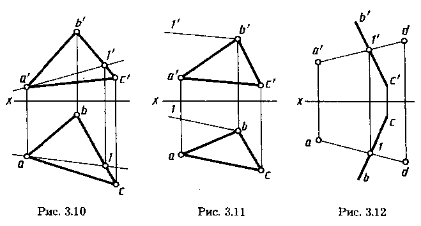
\includegraphics{img/321.png}\\


\subsection{Прямые особого положения плоскости-- главные линии плоскости}

Горизонтали(принадлежит плоскости и параллельна плоскости проекции H), фронтали(лежит в плоскости и параллельна фронтальной плоскости проекции), профильные(леж в плоскости и параллельна профильной плоскости проекции) прямые и линии наибольщего наклона.\\

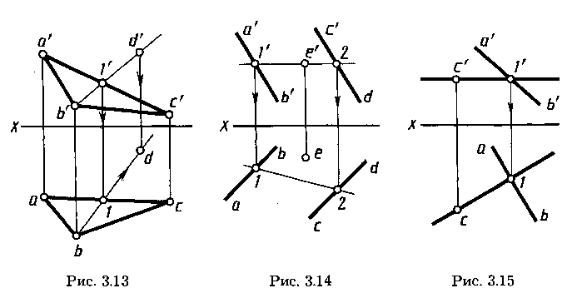
\includegraphics{img/331.png}\\
Линии наибольшего наклона  -- называют прямые лежащии в этой плоскости и перпендикулярные или к горизонталям или к ее фронталям или к ее профильным прямым\\

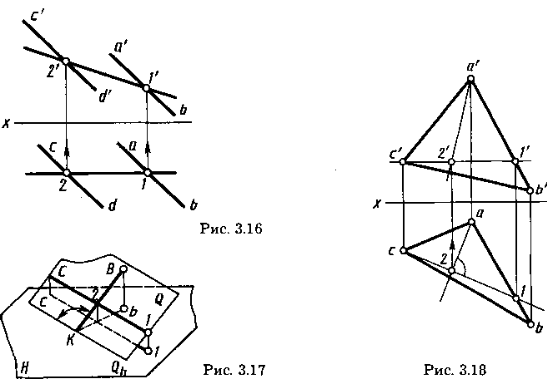
\includegraphics{img/332.png}\\


Угол между линией ската и ее горизонтальной проекцией является линейным углом между плоскостью, которой принадлежит линия ската, и плоскостью проекций Н\\

\section{ Глава. Взаимное положение прямой и линии в плоскости, двух плоскостей}

\subsection{Пересечение прямой линии с проецирующей плоскостью}

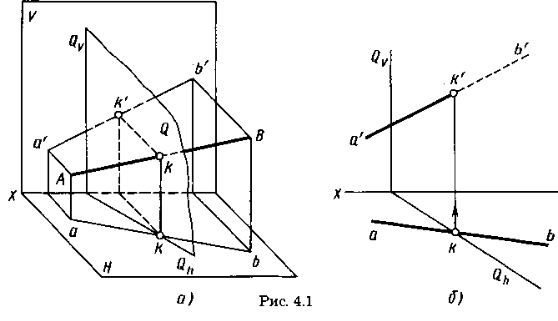
\includegraphics{img/411.png}\\


*для сложных чертежей анализ видимости мы не делаем*\\

Правила:\\
- Условно считают, что данная плоскость непрозрачна. Поэтому точки, линии, участки другой плоскости, расположенные между плоскостью проекций и данной плоскостью, невидимы для наблюдателя, между которым и плоскостью проекций находятся изображаемые объекты. Если линии, точки, участки другой плоскости находятся между данной плоскостью и наблюдателем, то они видимы и закрывают точки, линии, участки данной плоскости, лежащие на одних проецирующих прямых.\\

- Анализ видимости линий обычно проводят путем анализа видимости точек, как это сделано при анализе видимости конкурирующих точек на скрещивающихся прямых\\

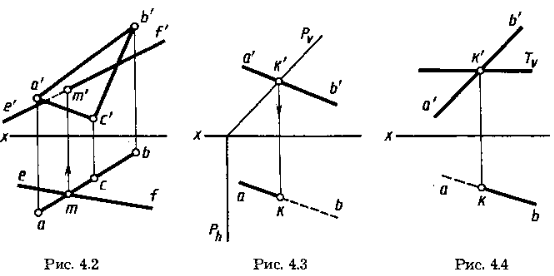
\includegraphics{img/412.png}\\


\subsection{Пересечение двух плоскостей}

*ДОСТАТОЧНО ПОСТРОИТЬ ОДНУ ТОЧКУ А ВТОРУЮ ТОЧКУ МОЖНО ПОЛУЧИТЬ ТАКИМ ЖЕ СПОСОБОМ*

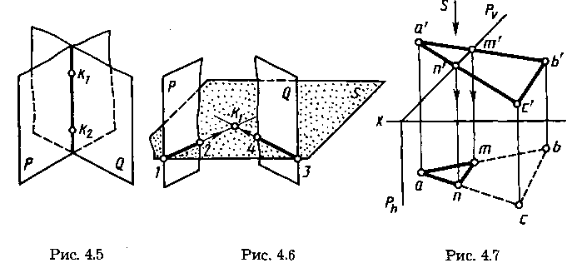
\includegraphics{img/421.png}\\

Для того чтобы найти точку принадлежащую двум плоскостям вводим вспомогательную плоскость строят линии пересечения вспомогательной плоскости с двумя заданными плоскостями и в пересечении построенных линий находят общую точку двух плоскостей. Для нахождения второй общей точки построение повторяют с помощью еще одной вспомогательной плоскости.\\

Частный случай построения линии пересечения двух плоскостей, когда одна из них проецирующая. В этом случае построение линии пересечения упрощается тем, что одна ее проекция совпадает с проекцией проецирующей плоскости на ту плоскость проекций, к которой она перпендикулярна.\\


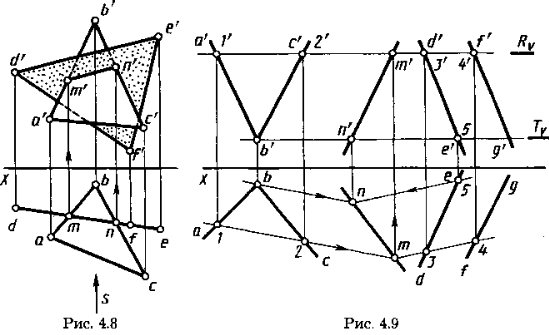
\includegraphics{img/422.png}\\
Построение линии пересечения плоскостей общего положения. На рисунке 4.9 приведено построение проекций т'п', тп линии пересечения двух плоскостей, одна из которых задана проекциями а'b', b'с’, ab, bс двух пересекающихся прямых, другая — проекциями d’e’, f'g', de, fg двух параллельных прямых.\\

Вспомогательные плоскости параллельны друг-другу.\\


\subsection{ Пересечение прямой линии общего положения с плоскостью общего положения}

Точку пересечения прямой с плоскостью общего положения строят в следующем порядке:\\
а)    через заданную прямую АВ проводят вспомогательную плоскость Т;\\
б)    строят линию пересечения 1—2 вспомогательной плоскости Т и заданной плоскости Q;\\
в)    в пересечении построенной линии 1—2 с заданной прямой АВ отмечают искомую точку К.\\

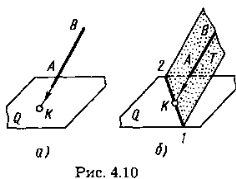
\includegraphics{img/431.png}\\

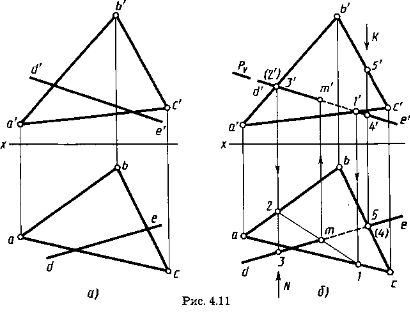
\includegraphics{img/432.png}

\subsection{ Построение взаимно-параллельных прямой и плоскости, двух плоскостей}
\subsubsection{Построение взаимно параллельных прямой линии и плоскости}

\quad \quad \quad \quad \quad \quad \quad 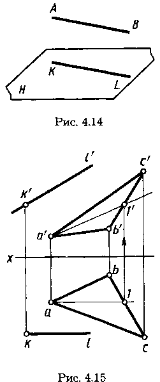
\includegraphics{img/441.png}\\

Для построения прямой, проходящей через заданную точку пространства параллельно заданной плоскости, достаточно провести прямую, параллельную любой прямой, принадлежащей плоскости.
При этом возможно бесчисленное множество решений. Дополнительные требования могут обусловить единственное решение.

Если необходимо проверить параллельна ли прямая заданной плосоксти нужно построить прямую параллельную заданной прямой в плоскости(если не существует -- то они не параллельны).

\subsubsection{Построение взаимно параллельных плокостей}

Если две пересекающиеся прямые, лежащие в одной плоскости, взаимно параллельны двум пересекающимся прямым лежащим в другой плоскости то плоскости параллельны.\\
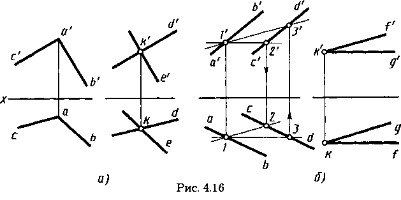
\includegraphics{img/442.png}\\

\subsection{Построение взаимно перпендикулярных прямой и плоскости}

\quad \quad \quad \quad \quad \quad \quad \quad 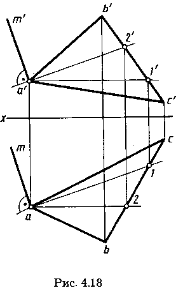
\includegraphics{img/451.png}\\
Если прямая перпендикулярна двум пересекающимся прямым, принадлежащим плоскости, то она перпендикулярна этой плоскости.\\

Чтобы построить две взаимно перпендикулярных плоскости необходимо построить перпендикуляр к одной из плоскостей а затем провести через одну из точек данного перпендикуляра  прямую, не принадлежащую исходной плоскости.

\subsection{Угол между прямой и плоскостью}
\quad \quad \quad \quad \quad \quad \quad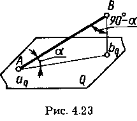
\includegraphics{img/461.png}\\
Угол между прямой и плоскостью определяется углом между этой прямой и ее проекцией на плоскости. Для решения этой задачи требуется:\\
1) найти точку пересечения прямой с плоскостью\\
2) провести из некоторой точки прямой перпендикуляр на плоскость.\\
3) определить точку пересечения перпендикуляра с плоскостью.\\
4) соединить эти точки линией\\\
5) определить угол между прямой и плоскостью\\
Ообычно достаточно построить только перпендикуляр. Задача определения угла между двумя прямыми расматривалась нами когда мы решали задачу определения угла наклона прямой к плоскости.

\section{Глава. Способы преоброзования чертежа}
\subsection{Общая характеристика способов преоброзования чертежа}

Многие задачи рашаются легко если линии и плоскии фигуры, образующие объект находятся в частном положении. Такого добится позволяет преоброзование чертежа, добится которого позволяют пару способов:\\
1) Переменной плоскостей проекции(в этом случае заданную систему плоскостей и проекций заменяют на новую так, чтобы исходные объекты не меняя своего положения в пространстве оказались в частном положении).\\
2) Способ вращения(в этом случае не измения плоскостей проекции исходные объекты поварачивают таким образом, чтобы они приняли частное положение).\\

\subsection{Способ перемены плоскостей проекции}
-- при этом способе преоброзовании чертежа положение точек, линий, плоских фигур, поверхностей в пространстве не изменяется, а система VH дополняется плоскостями, образующими с V или H или между собой систему двух взаимно перпендикулярных плоскостей, принемаемых за плоскости проекции.\\
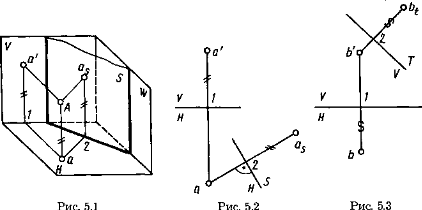
\includegraphics{img/521.png}\\

Можно проводить несколько раз.\\

4 основные задачи преобразования:\\
1) определение величины отрезка общего положения.\\
2) приведение плоской фигуры общего положения в проуцирующее положение.\\
3) Определение натурального вида плоской фигуры, расположенной в проецирующем положении.\\
4)Приведение отрезка прямой общего положения в проецирующее положение.
%Отредактировать изображения
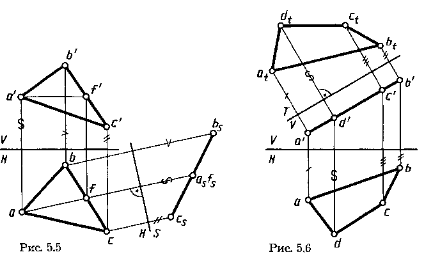
\includegraphics{img/522.png}\\
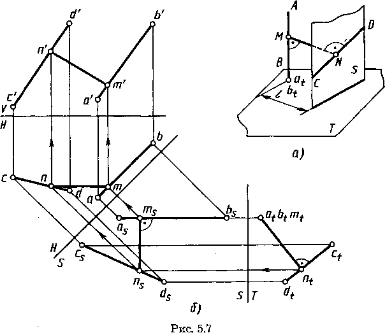
\includegraphics{img/523.png}\\
с помощью переменной плоскостей проекции можно определять растояние, это растояние представляет собой длинну общего перпенидкуляра,его длину удобно определять когда одна из скрещивающихся прямых находится в проецирующем положениию, таким образом мы вводим новую плоскость проекций такую,в которой одна из прямых находится в проецирующем положении, строим перпендикуляр ко второй прямой и определяем его длину.\\

\subsection{Способ вращения}

чтобы применить преобразование чертежа необходимо задать  несколько элементов:\\
1. ось вращения\\
2. плоскость вращения точки\\
3. центр вращения\\
4. радиус вращения(растояние от центра вращения до точки)\\
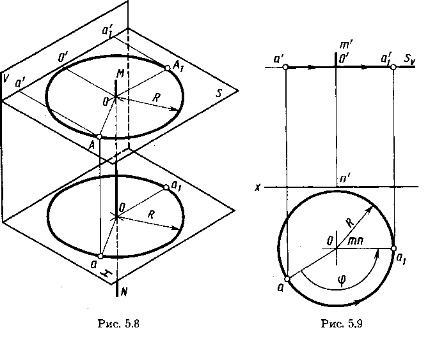
\includegraphics{img/531.png}\\

В качестве оси вращения обычно используют прямые, перпендикулярные или параллельные плоскостям проекций. Она может быть прямой общего положения но на практике не применяется.\\

Вращение точки A относительно MN, перпендикулярной относительно плоскости проекции.\\
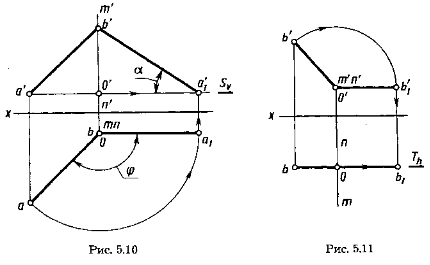
\includegraphics{img/532.png}\\

Вращение вокруг прямых параллельных плоскостям проекции\\
-- Натуральную велечину фигуры можно определить вращением вокруг оси параллельной плоскости проекции. В этом случае одним поворотом фигура приводится в плоскость параллельную плоскости проекции.\\

\section{Изображение многогранников}
\subsection{Применение многогранников в технике}
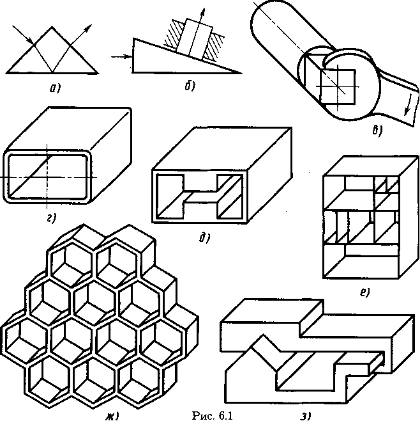
\includegraphics{img/611.png}\\
\subsection{Чертежи призмы и пирамиды}
Грани призмы и пирамид ограничиваются ребрами, а ребра представляют собой прямолинейные отрезки, которые пересекаются между собой, поэтому построение чертежей призмы пирамидсводится к построению точек(вершин) и отрезков прямых(ребер).\\

Призматическая поверхность может быть представлена на чертеже проекциями ребер или проекцией фигуры, которая получается при пересечении боковых граний плоскостью. Пересекая призматическую поверхность двумя параллельными плоскостями получают основание призмы. На чертеже основания призм удобно распологать параллельно плоскостям проекции.\\

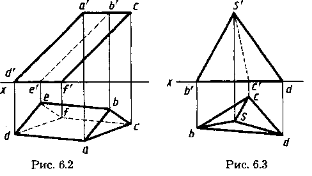
\includegraphics{img/621.png}\\

Одноименные проекции ребер призмы параллельны между собой.\\
Пирамиду создает основание ребер и её вершин.

\subsubsection*{Призмы и пирамиды в трех проекциях. Точки на поверхности}
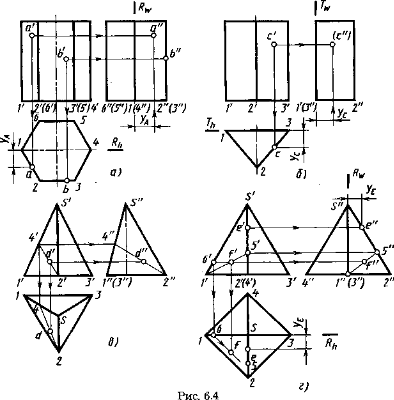
\includegraphics{img/622.png}\\

\subsection{Определение высоты пирамиды}

Высота пирамиды -- растояние от вершины до плоскости основания.\\
Если пирамида состоит из участков плоскостей общего положения, то определение её высоты проводится с помощью способы перемены плоскостей проекции. Новая плоскость проекций выберается перпендикулярной прямой частного положения проходящей через точку пересечения перпендикуляра к плоскости основания пирамиды опущенного из её вершин, т.е:\\
1) строим перпендикуляр из вершины пирамиды к плоскости её основания.\\
2) проводим через эту точку линию частного положения лежащего в плоскости основания пирамиды.\\
3) перпендикулярно этой линии вводим новую плоскость проекции.\\
4) искомая высота пирамиды будет найдена как длина проекции на эту плоскость перпендикуляра, построенного на первом шаге.\\

\subsection{Пересечение многогранников плоскостью}

При пересечении призмы или пирамиды плоскостью, в сечении получается плоская фигура, ограниченная линиями пересечения секущей и плосостью с гранями призмы или пирамиды.\\
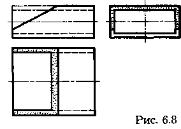
\includegraphics{img/641.png}\\
\subsubsection*{Определение натурального вида сечения пирамиды плоскостью}
Для определения натурального вида сечения плоскостью можно использовать метод переменны плосокстей.\\
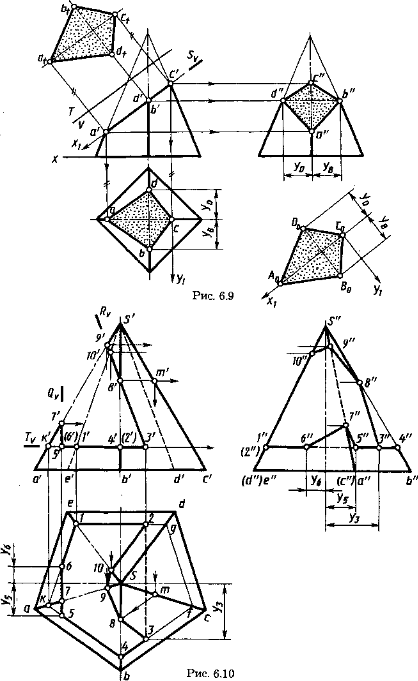
\includegraphics{img/642.png}\\


\subsection{Построение точек пересечения прямой с поверхностью многогранника}
Чтобы построить точки пересечения поверхности многогранника какой-либо прямой сначало необходимо найти пересечение этого многогранника проецирующей плоскостью, в которой лежит эта прямая.\\
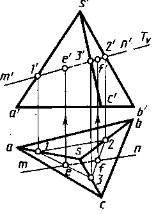
\includegraphics{img/643.png}\\

\subsection{Развертка гранных поверхностей}
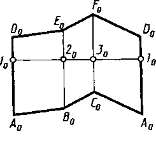
\includegraphics{img/661.png}\\
Разверткой поверхности многогранника называют плоскую фигуру полученную при совмещении с плоскостью всех его гранней. Развертывание гранных поверхностей выполняют для проведения раскроя листового материала при изготовлении детали или для определения площади поверхности детали покрываемых различными покрытиями(не только декаративные, но и защитные или придающие поверхности материала заданные свойтсва). Для построения развертки необходимо определить размеры граней многогранника. Универсальный способ, пригодный для любого многогранника -- грань разбивается на треугольники, а натуральный вид треугольников оопределяется любым из ранее расмотренных методов.\\

\section{Глава. Аксонометрические поверхности}

\subsection{Аксонометрические поверхности как способ представления детали}
Способ аксонометрического проецирования состоит в том, что данная фигура вместе с осями прямоугольных координат, к которым она отнесена в пространстве, проецируется параллельно на некоторую плоскость принятую за плоскость аксонометрических проекций, эту плоскость также называют картинной плоскостью.\\

Прямоугольные аксонометрические проекции оси присоединненных прямоугольных координат к детали распологают не параллельно к плоскости аксонометрических проекций.\\

Аксонометрических проекций существует бесконечное множество. Они будут отличатся направлением осей.\\

\subsubsection*{Коэфицент искажения}
\[
	\cos^2 \alpha + \cos^2 \beta + \cos^2 \gamma = 2
\]

\subsection{Изометрическая проекция}

На практике применяют коэфицент искожения = 1, его называют приведенным коэфицентом искажения

\subsection{Демитрическая проекция}

\newpage
\section{Глава. Изображение предметов.\\Виды,разрезы,сечения}

\subsection{Основные положения}
При ортогональном проецировании внешний вид объекта проецируется на три плоскости проекции.Таким образом мы полючаем три плоских изображения для объемного предмета.Во многих случаях их достаточно для получения общего представления об объекте.\\

Для сложных деталей могут потребоватся дополнительные изображения. Правило изображения на чертежах изложенны в стандартах, входящих в систему конструкторской документации.\\

Предметы на чертежах изображаются методом прямоугольной проекции и не как по другому при этом предпологается что ихображаемый предмет распаложен между наблюдателем и плоскостью проекции. Такой метод называется методом первого угла или методом 'E'.За основные плоскости проекций принемают шесть граней куба.\\

Изображением является любой чертеэ который может быть видом,разрехзом или сечением.Ихображение выполняется установленном образом проецирования в определенном маштабе.\\

Главное ихображение - это главное ихображение на плоскости проекции. Обхект рапологают на фронтальной плоскости поверхности так чтобы ихображение на ней давало наиболее полное представлени о форме и размерах предмета.\\

Предметы следует ихображать в функциональном положении или в положении удобном для ихготовления. Предметы состоящии их нескольких частей всегда ихображают в функциональном положении.\\

Предметы используемые в любом положении ихображают в любом положении удобном для изготовления. А предметы функциональное положение которого наклонное изображают в вертикальном или горизонтальном положении.\\

Длинные или выскоие предметы функциональное положение которых вертикальное можно изображать в горизонтальном положении но нижнюю часть предмета следует помещать справа.\\

Вид -- это изображени обращенной к наблюдателю видимой части поверхности предмета.\\
Разрез -- изображение предмета мысленно расеченного одной или несколькими плоскостями. При этом рассечение предмета относится только к данному разрезу и не влечет за собой изменений других изображений тогоже предмета. На разрезе показывают то что получается в секущей плоскости и что расположенно за ней. Секущую плоскость выбирают так чтобы получить наиболее полное представление о предмете. Та часть разреза обозначающая разрез обозначается штриховкой.\\
Сечения отличаются тем что на них ихображенна фигура получающаяся при рассечении предмета секущей плоскостью в отличии от разреза на сечении не изображают то что находится за секущей плоскостью.\\



\subsection{}

Для видов установленны названия:\\
1) вид спереди(главный)\\
2) вди сверху\\
3) вид слево\\
4) вид справо\\
5) вид снизу\\
6) вид сзади\\

Если расположение видов соотвествует рассмотренному в предыдущем параграфе то подписывать виды ненужно. Если есть необходимость сместить какой-то из видов .
Если нет изображение на котором .Для уменьшения кол-ва видомв допускается невидимые контура изображать штриховой линией.\\

Если какую либо часть предмета невозможно нарисовать на основных видов юбех искажени формы и размеров то применяют дополнительные виды которые строят на плоскостьях не параллельных плоскостям проекции. Дополнительный вид указывается стрелкой в раплавлении взгляда и подписывается заглавной буквой русского алфавита.\\

Местный вид -- изображения местной поверхности предмета. Отмечают его также как дополнительный вид.\\

Сложные разрезы бывают ступенчатые и ломанные. \\
Ступенчатыми называют разрезы у которых секущии плоскости параллельны.\\
Ломаным называется разрез когда секущие плоскости пересекаются.\\

Местный разрез -- это разрез который служит для выявления формы предмета в отдельном месте. Местный отделяют от вила сплошной волнистой линией. Она не должна совподать с какими либо любыми видами изображения.\\

\subsection{Сечения}

Сечения не входящие в состав разреза бывают двух видов: вынесенные и наложенные. При этом вынесенное сечение является предподчтительней. Их допускается распологать в разрыве предмета.\\

Контур вынесенного сечения изображают сплошной основной линией а контур наложенного сечения тонкой линией. Для наложенных сечений и наложенных в разрезе указывают направление взгляда но не подписывают.\\

\section{Глава. Некоторые положения конструкторской документации}
\subsection{Нормативно технический документ}
Создание промышленных изделий начинается с контрукторской документации. Она всегда выполняется с соответствии с требованиями стандартов.
\\Стандарты:\\
Гост 1. - ГСС\\
Гост 2. - ЕСКД\\
Гост 3. - ЕСТД\\
Структура: ГОСТ Р(если распада после СССР) 2.ххх-хх\\
ОСТ\\
ТУ\\

\subsection{Виды изделий}
Изделие - это любой предмет или набор предметов подлежащий изготовлению. Виды изделий установлены ГОСТ 2.101-68. Согласно стандарту сузествуют виды изделий: деталь(изделие изготовленное из однородного по наименованию и марки матерьияла без пременения сборочных операций),сборочная единица(изделие состовные части которого подлежат соединению между собой на предприятии изготовителя сборочными операциями), комплеск(два и более изделий состоязих в свою очередь каждая из двух и более частей не соединенных сборочными операциями на предприятии изготовителя но предназначенны для управления взаимосвязанных эксплатуационных функций),комплект(два и более изделей не соединненых сборочными операциями но имеющих общее эксплуатационное назначение).\\

\subsection{Стадии разработки конст. документации и виды конст. документов}

Разработка КД детали начинается с определения технического предложения. Оно разрабатывается в соотвествии с технич заданием заказчика. Иногда по итогам подготовки технич предложения техн задание приходится корректировать.\\

Эскизный проект выполняют для установления принципиальных решений дающих общее представлении о работе и устройстве изделия. По искизной документации изготавливают и испытывают макет. \\

Техническом проекте принемают окончательное решени с подробной изготовкой общих видов чертежей и деталей и схем изделия позволяюзих оценить соотвествие изделия требованиям технического задания технологичность и т.п. На этапе техн проекта используются все наработки полученные ранее.\\

Рабочая конструкторская документация используется для разработки и изготовления опытного образца устанновочной серии и массовой серии изделия. Стадии разработки обозначаются с помощью литеров(П,Э,Т,О,А,Б).

К конст док относятся графические и текстовые документы которые определяют состав и устройство изделия и содержат необходимые данные для его разработки изготовления приема контроля приемки экстплуотации и ремонта. Также подразделяются на проектные и рабочие(чертеж детали или сборочный чертеж(литеры - СБ)). Спецификация - документ определяющий состав сборочной единицы или документа(АААА.ХХХХХХ.УУУ.ZZ). 

Графические документы: габаритный чертеж(ГЧ), электромонтажный чертеж(МЭ), монтажный чертеж(МЧ), упоковочный чертеж(УЧ), схемы - документы на которых состовные части изделий показанны в виде условных изображений(ГОСТ 2.701-84): виды обозначаются буквой(э - электрические,г-гидравлические,п-пневматические,к-кинематические и т.д) и типы схем: %что-нибудь написать
.\\

Текстовые документы: технические условия(ТУ), патентный формуляр(ПФ), инструкция(И), ведомость(ПЭ3,ВП).


\subsection{Содержание чертежа или искиза детали}
Под чертежом детали понимают основной конструкторский документ содержащий изображение детали и другие данные необходимые для ее изготовления и контроля.
Помимо формы и размеров детали рабочий чертеж в общем случае содержит еще ряд сведенний:\\-- предельное отклонение размеров, формы и поверхности;\\ -- обозначение широховатости поверхности;\\ -- обозначение покрытий и видов обработки детали;\\ -- текстовую часть состоящую из технических требований и характеристик детали.\\

Рабочие чертижы изготавливают на каждую деталь. Стандартом допускается не изготавливать рабочии чертежы на некоторые виды деталий(детали изготавлевыемые из фасонного материала отрезкой под прямым углом и из листового материала  резкой по окружности).

Если для детали по условиям сборки изделия или условиям расположения деталий в изделии важны размеры в напряженном состоянии, то  на чертеже изображают деталь в двух состояниях(в свободном сплошными линиями, в напряженном штрих-пунктирными линиями). Соответсвенно размеры наносятся для того и другого случая. Если деталь в свободном состоянии приобретает произвольную форму которую на чертеже не указывают , то такую деталь указывают только в напряженном положении.

\subsection{Выбор изображений и планировка искиза или чертежа}
Если деталь представляет собой тело вращения то для нее достаточно одного изображения на плоскости проекций параллельной оси тела. Также достаточно для валов, втулок и т.д. . Елси деталь представляет собой тело вращения но имеет конструктивные элементы, то главное изображение дополняют однним или несколькими методами, которые позволяют выявить их. Для тонких плоских деталий также достаточно одного изображения.

Главное изображения выбирают с учетом изготовления детали. Если в процессе изготовления одно из ее положений является приобладающим то на главном изображении деталь нужно показывать в этом положении. При этом планки распалагают горизонтали, а корпусы основанием вниз. Если деталь сложной конструкции не имеет преоблодающего изображение, то за главное изображение принимают деталь в готовом изделии. Для диталий типа шкива и колес главным изображением является фронтальный разрез(он выевляет внешние очертания детали, поэтому вида спереди не требуется). В этом случае разрез выполняют полностью. Крепежные элементы изготавливаются на токарных станках или автоматах. Ось этих деталий почти всегда горизонтальна.

Формат чертежа или искиза выбирают в зависимости от сложности и размеров детали, при этом необходимо учитывать возможные изменения маштаба. Мелкие сложные датали дают с увеличением, а простые крупные детали чертят в уменьшенном размере. Для мелких елементов детали используют выносные элементы. Прежду чем выбрать формат чертежа необходимо осмотреть деталь и определить неоходимое кол-во видов. На предварительно выбранном формате выполняют черновик планировки чертежа, на котором чертят осевые линии и их габаритные контуры, а также отмечают зоны изображения размеров. А затем оценивают можно ли уменьшить формат листа.

\subsection{Нанесение размеров на эскизах и чертежах деталей}
1) Общее положение\\
Величину изображаемого предмета и его элементов определяют размерные числа нанесенные на чертеже. Нужно учитывать форму детали, взаимодействие детали с другими деталями, особенности изготовления детали, обеспечение ясности и выразительности чертежа.\\

2) Обеспечение ясности и выразительности чертежа.\\
Размеры на чертеже указывают размерными линиями и числами. Линии выполняют в виде прямолинейного отрезка или в виде дуги окружности с одной или двумя стрелками. Числа без обозначения единиц измерения указывают размер в милиметрах. Другие единицы измерения необходимо указывать. Угловые размеры в градусах,минутах и секундах. Кол-во изображений должно быть минимальным но достаточным. Повторение размеров не допускается на разных изображениях. Размеры предпочтительно наносить вне контура изображения. При нанесении выносных и размерных линий необходимо избегать их пересечений. Чертижы симетричных предметов иногда чертят только до оси симетрии. В этом случае выносные линии проводят с обрывом и этот обрыв делают дальше оси симетрии.
Размеры относящиеся к одному материалу рекомендуется компоновать в одном месте, расопологая на том изображении, на котором показано наиболее полно.
Размеры внутренних в внешних очертаний детали лучше делать отдельно. Стрелки равны. Если длины размерной линии для стрелки недостаточно, то стрелки размещают снаружи. Если размеры следуют цепочкой, при нехватки места разрешается заменять стрелки засечками под углом 45 градусов. Размерные числа наносят над размерной линией ближе к ее середине(искл.-- рисование диаметра внутри окружности). Если раз. линии идут параллельно друг-другу то рекомендуется распологать числа в шахматном порядке(и угловые размеры).\\
Правила:\\
1) размерные числа недопускается пересекать. В местах нанесения линии прирывают\\
2) недопускается разрывать линию контура для нанесения размерного числа\\
3) не наносят разм. числа в местах пересечения размерных осевых или центровых линий\\

\subsection{Надписи и обозначения на чертежах}

На поле рабочего чертежа наряду с уже расм изобр изделия его размерами и обозначениями приводят обозначения допускаемых отклонений, размеров формы и расположения поверхностей, их широховатости, а также различные надписи, тех требования и таблицы.

1) Надписи на чертежах\\
Их выполняют в том случае если в тексте данные указания невозможны или нецелесообразно выразить графически. Содержание должно быть кратким и точным. Надписи выполняют без сокращений( кроме обще принятых -- ГОСТ 2316-68 ). Текста на поле чертежа распологают параллельно основной надписи. Около изображений на полках линий выносок наноссят только краткие надписи относящиеся к изображения предмета. Линию выноску пересекающую контур изображения заканчивают точкой. Линию выноску отводимую от линии видимого и невид контура заканчивают стрелкой. На конце линии выноски от всех других линий недолжно быть ни стрелки ни точки. ИХ проводят так чтобы они не пересекались между собой. Если она проходит по заштрихованному полю следуте проводить не параллельно штриховки. Она не должна пересекать размерные линии и элементы изображения, к которым она не относится.\\
Надписи которые относятся непосредственно к изображению не могут содерж не более двух строк. Если тербуется поместить более объемный текст его помещают над основной надпистью. Между текстовой надписью не позволяется помещать текст или таблицу. Текст чать содержит описание тех требования. ПО возможности приволить эти требования следует в таком порядке:\\
1) тербования предъяв к материалу заготовки терм обработки и ксвойствам материала готовой детали\\
2) размеры предельные откланения размеров формы взаимного расположения поверх массы и т.д\\
3) требования к качеству поверхности указания об их отделки и покрытии\\
4) зазоры и расположения отдельныз элементов конструкции\\
5) другие требования к качеству изделий\\
6) требования предъявляемые к настройке и регулир изделия\\
7) условия и методы испытаний\\
8) указания маркировки и клеймении\\
9) правила транспортирования и хранения\\
Пункты должны иметь сквозную нумерацию и с новой строки. Заголовок не пишут.\\

Технические требования ко многим изделиям сформулированны к отраслевым стандартам(принем отраслевым министерством и явл обяз для подконтрольных предприятий) или стандартам предприятия(прин придприятием и соблюдается имже).

Если для изделия таблица параметров установленна стандартом, то ее помещают по правилам стандарта. Все другие таблицы размещают на свободном месте справа от изображения или ниже.

2) Нанесения предельных отклонений\\
Рассмотренные выше разрмеры называют нанминальные. Они находятся в ходе расчетов прочности и жесткости. Также руководствуются конструктивными или технологическими соображениями. Однако действительные значения размеров могут отличчатся от наминальных по многим причинам. Во первых оборудования работает неточно. В овторых все инструменты и присобления характерезуются погрешностью всегда а вдобавок часто имеют износ. В третиих в процесси ихготовления детали производятся силовые и температурыне деформации. При конструировании при расчете наминальных размеров необходимо установить и придельные значения размеров которые дожны быть угодной деталиили изделия. При этом как наибольшмй так и наимегьшей придельные размеры могуть быть больше наминального размера. Либо который их них может быть равен наминальному.

На машинастроительных чертежах проставляют в милиметрах. Верхнии отклонения указывают немного выше а нижнии немного ниже наминального размера и дают боллее мелким шривтом. 

\subsection{Спецификация}
-- Это конструкторский документ который содержит перечень всех составных частей входящих в данное изделие а также конструкторских документов к нему относящихся. Форма и порядок осуществляется в соответскии   с гостом. Ее выполняют на отдельных листах, причем основная надпись первых и последующих листов отличаются. Она представляет собой таблицу которая разделена на несколько разделов:\\
1 раздел -- Документация(все документы относящиеся к изделию)\\
2 раздел -- Сборочные единицы(обозначения и наименования входящих в изделие сборочных единиц)\\
3 раздел -- Детали(обозначения и наименования деталий которые входят в изделие непосредственно)\\
4 раздел -- Стандартные изделия(Указываются в алфавитном порядке; сначало крепежные а затем электрич и радиодетали)\\
5 раздел -- Прочие изделия(в алфавитном порядке)\\
6 раздел -- Материалы(если используются; Металы черные - магнитные - цветные металлы - благородные металлы - кабели провода и шнуры - пласмассы и пресованные материалы - бумага и текстиль - резина и кожевенные изделия - керамика и стекло - лаки и краски - т.д.; сорт в алф порядке)\\

Документы приводятся с указанием формата. Для сбор единиц и деталий указывается кол-во использованных элементов. Для этих объектов в примечании указывается буквенно-цифровые обозначения соотвествующие месту использования на принципиальной схеме. ДЛя материалов указывается кол-во масса или длина. Допустимо в качестве кол-во деталий указывать дробные числа.\\

\subsection{Общии понятия об оформлении схемы}
-- это документ в котором показаны в виде условных обозначений части изделия и связи между ними. Наиболее часто в практике разработки радиоэлектронных устройств используется электрическая принципиальная схема(Э3)(Гост 2701-84). Они выполняются без соблюдения маштабов.На схемах применябтся три способа графического оформления:\\
1) элементы схемы изображаются условными графическими обозначениями(Стандартизованны). ДЛя каждого вида схем они свои.\\
2) отдельные элементы схемы изображаются геометрическими фигурами (как правило квадратами) и отображаются связи между ними(стандартизованны).\\
3) элементы схем изображаются упращенными внешними очертаниями.\\

Правила:\\
- Условные граф обозначения указ в размерах установленных в стандартах. Если нет стандартных обозначений, то примененные обозначения выполняются в размерах приблизительно равном стандартным.\\
- Услов граф обознач допускается поворач на угол кратный 45 градусов или отражать зеркально. Размеры и толщену линий делают одинаковой на всех изображениях изделий. Линии связи должны состоять из горизонтальных и вертикальных отрезков. Кол-во изломов должно быть минимально возможных.\\

\subsection{Оформление электрической принципиальной схемы}
-- это документ определяющий полный состоав электрических элементов изделия. Схема дает представление о принципах работы изделия. Служит основой для разработки конструкции и используется при изготовлении и эксплуатации изделия. Схема в обязательном порядке содержит перечень элементов.\\
Элементы изображают совмещенным(сост части показ на схеме в непосред близости) и разнесенным(в разных местах) способами. Второй способ затрудняет чтение схемы но облегчает понимание принципов ее работы. Для упращения схемы иногда эл несвяз линии группируют в одну общую. Обычно это используется для отображения шин(в особенности параллельных).\\
Для однозначного определения элементов им присваивают буквенно-цифровые обозначения(гост 2710-81). Оно состоит из трех частей(вид,порядковый номер предела данного вида,функциональное назначение)




\end{document}